\documentclass{beamer}
\usepackage[spanish]{babel}
\usepackage[latin1]{inputenc}
\usepackage{multicol} % indice en 2 columnas
\usepackage{centernot}
\usepackage{amsmath}% http://ctan.org/pkg/amsmath

\usepackage{color}


\usepackage{graphicx}
\graphicspath{ {im/} }


\newcommand{\notimplies}{%
  \mathrel{{\ooalign{\hidewidth$\not\phantom{=}$\hidewidth\cr$\implies$}}}}


\usetheme{Warsaw}
%\usecolortheme{crane}
\useoutertheme{shadow}
\useinnertheme{rectangles}

\setbeamertemplate{navigation symbols}{} % quitar simbolitos


\title[Tema 3 - Espacios vectoriales]{Espacios vectoriales}
\subtitle{Estudios de Ingenier\'ia}
\author[https://frogames.es]{
Juan Gabriel Gomila%$^{1}$  \and E. Eva$^{2}$ \and S. Serpiente$^{3}$
}
\institute[Frogames]{
 % $^{1-2}$
 Frogames
   \and
  \texttt{https://frogames.es}
}
\date{\today}


\AtBeginSection{
\begin{frame}
  \begin{multicols}{2}
  \tableofcontents[currentsection]   
\end{multicols}
\end{frame}
}

\AtBeginSubsection{
\begin{frame}
  \begin{multicols}{2}
  \tableofcontents[currentsection,currentsubsection]
\end{multicols}
\end{frame}
}



%empieza aqui


\begin{document} 

\frame{\titlepage}

\begin{frame}
  \frametitle{\'Indice}
  \tableofcontents
\end{frame}

\section{Conjuntos libres y ligados}
\subsection{Combinaciones lineales}

\begin{frame}
  \frametitle{Combinaciones lineales}
  \begin{block}{Combinaci\'on lineal}
Recu\'erdese que dados $p$ vectores $\vec u_1,\vec u_2,\cdots,\vec u_p\in\mathbb K^n$ y los escalares $\alpha_1,\alpha_1,\cdots,\alpha_p\in\mathbb K$ una combinaci\'on lineal de esos $p$ vectores es un vector dado por una expresi\'on de la forma:
\[\alpha_1\vec u_1+\alpha_2\vec u_2+\cdots+\alpha_p\vec u_p\in \mathbb K^n\]
\end{block}

\begin{block}{Ejercicios}
Expr\'esese el vector $(2,-4)$ como una combinaci\'on lineal de los vectores $(1,1)$ y $(-2,0)$.
\end{block}
Sol:$(2,-4) = -4(1,1)-3(-2,0)$.
\end{frame}

\begin{frame}
  \frametitle{Combinaciones lineales}
  \begin{block}{Ejercicios}
Expr\'esese el vector $(4,-11)$ como una combinaci\'on de los vectores $(2,-3)$ y $(4,-6)$.
\end{block}
Sol: no tiene soluci\'on.
\begin{block}{Ejercicios}
Expr\'esese el vector $(4,-11)$ como una combinaci\'on de los vectores $(2,-1)$ y $(1,4)$.
\end{block}
Sol:$(4,-11) = 3(2,-1)-2(1,4)$.
\begin{block}{Ejercicios}
Pru\'ebese que el vector $(1,0)$ no se puede expresar como una combinaci\'on lineal de $(2,-3)$ y $(4,-6)$
\end{block}
\end{frame}

\begin{frame}
  \frametitle{Combinaciones lineales}
  \begin{block}{Ejercicios}
Expr\'esese el vector $(4,-5,6)$ como una combinaci\'n lineal de los vectores $(2,-3,5)$ y $(-1,3,2)$.
\end{block}
Sol: no tiene soluci\'on
\begin{block}{Ejercicios}
Expr\'esese el vector $(4,-5,7)$ como una combinaci\'on lineal de los vectores $(0,-3,5),(1,0,-3)$ y $(-1,3,4)$.
\end{block}
Sol:$(4,-5,7) = \frac{31}{9}(0,-3,5)\frac{52}{9}(1,0,-3)+\frac{16}{9}(-1,3,4)$.
\begin{block}{Ejercicios}
Expr\'esese, si es posible, el vector $(0,0,0)$ como una combinaci\'on lineal de $(-1,3,1), (1,0,-3)$ y $(-1,3,4)$, distinta de $(0,0,0)$.
\end{block}
\end{frame}


\begin{frame}
  \frametitle{Dependencia e independencia lineal}
  \begin{block}{Dependencia lineal}
Dados el conjunto ed vectores $\vec u_1,\vec u_2,\cdots,\vec u_p\in\mathbb K^n$ d\'icese que son linealmente dependientes si alguno de ellos se puede expresar como una combinaci\'on lineal del resto. Son LD si:
\[\exists 1\leq i\leq p\ : \ \sum_{k\neq i} \alpha_k \vec u_k = \vec u_i\]
\end{block}
\end{frame}


\subsection{Dependencia e independencia lineal}
\begin{frame}
  \frametitle{Dependencia e independencia lineal}
  \begin{block}{Ejercicios}
D\'igase si el conjunto de vectores $(2,-4,0), (1,1,1)$ y $(-1,2,0)$ es linealmente dependiente.
\end{block}

\begin{block}{Ejercicios}
D\'igase si el conjunto de vectores $(-1,6,5), (1,0,-3)$ y $(-1,3,4)$ es linealmente dependiente.
\end{block}
\end{frame}


\begin{frame}
  \frametitle{Dependencia e independencia lineal}
  \begin{block}{Independencia lineal (II)}
Dado el conjunto de vectores $\vec u_1,\vec u_2,\cdots,\vec u_p\in\mathbb K^n$ d\'icese que son linealmente dependientes si la ecuaci\'on vectorial
\[\sum_{i=1}^p \alpha_i \vec u_i = \vec 0\]
tiene infinitas soluciones, y por tanto los escalares $\alpha_i\in\mathbb K$ pueden tener valores no nulos.
\end{block}
  \begin{block}{Ejercicios}
D\'igase si el conjunto de vectores $(2,-4,0), (1,1,1)$ y $(-1,2,0)$ es linealmente dependiente.
\end{block}

\end{frame}




\begin{frame}
  \frametitle{Dependencia e independencia lineal}
  \begin{block}{Independencia lineal}
Dado el conjunto de vectores $\vec u_1,\vec u_2,\cdots,\vec u_p\in\mathbb K^n$ d\'icese que son linealmente independientes si no es posible expresarlos como una combinaci\'on lineal del resto. Son LI si:
\[\not\exists 1\leq i\leq p\ : \ \sum_{k\neq i} \alpha_k \vec u_k = \vec u_i\]
\end{block}
  \begin{block}{Ejercicios}
D\'igase si el conjunto de vectores $(2,-4,0), (1,1,1)$ y $(-1,2,1)$ es linealmente independiente.
\end{block}


\end{frame}



\begin{frame}
  \frametitle{Dependencia e independencia lineal}
  \begin{block}{Dependencia lineal (II)}
Dado el conjunto de vectores $\vec u_1,\vec u_2,\cdots,\vec u_p\in\mathbb K^n$ d\'icese que son linealmente independientes si la ecuaci\'on vectorial
\[\sum_{i=1}^p \alpha_i \vec u_i = \vec 0\]
tiene como \'unica soluci\'on la soluci\'on trivial, es decir $\alpha_i=0\forall 1\leq i\leq p$.
\end{block}
  \begin{block}{Ejercicios}
D\'igase si el conjunto de vectores $(2,-4,0), (1,1,1)$ y $(-1,2,1)$ es linealmente independiente.
\end{block}
\end{frame}

\begin{frame}
  \frametitle{Dependencia e independencia lineal}
  \begin{block}{Ejercicios}
Demu\'estrese que el conjunto $(1,1)$ y $(1,0)$ es LI.
\end{block}
  \begin{block}{Ejercicios}
Demu\'estrese que el conjunto $(1,1)$ y $(0,1)$ es LI.
\end{block}
  \begin{block}{Ejercicios}
Demu\'estrese que el conjunto $(1,1),(1,0)$ y $(0,1)$ es LD.
\end{block}
\end{frame}


\subsection{Rango de un conjunto de vectores}
\begin{frame}
  \frametitle{Rango de un conjunto de vectores}
  \begin{block}{Definici\'on}
Dado el conjunto de vectores $\vec u_1,\vec u_2,\cdots,\vec u_p\in\mathbb K^n$, d\'icese que tienen rango $r\leq p$ si existe como m\'inimo un subconjunto de $r$ vectores linealmente independientes entre ellos y no existe ninguno de $r+1$ vectores que sea linealmente independiente. Es decir, es el n\'umero m\'aximo de vectores linealmente independientes que pueden extraerse del conjunto.
\end{block}
  \end{frame}



\begin{frame}
  \frametitle{Rango de un conjunto de vectores}
  Un m\'etodo para calcular el rango de un conjunto de vectores consiste en construir una matriz utilizando los vectores como columnas (o filas) y definir el rango de la matriz como el rango de sus vectores columna (o fila). Ya se ha aprendido c\'omo calcular el rango de una matriz en el Tema 1. Ahora se pondr\'a en pr\'actica para calcular el rango de vectores.
  \begin{block}{Definici\'on}
El rango de una matriz $A$ coincide con el n\'umero de vectores fila o columna linealmente independientes. 
\end{block}
    \end{frame}


\section{Espacios vectoriales de dimensi\'on finita}
\subsection{Espacios vectoriales}
\begin{frame}
  \frametitle{Espacios vectoriales}
  Hasta ahora se han visto ejemplos de espacios de $\mathbb R^2$ y $\mathbb R^3$, pero la gran mayor\'ia de definiciones que se han presentado se han dado para espacios $\mathbb K^n$ arbitrarios. Veremos que la estructura de estos espacios es una de las m\'as importantes en el mundo del \'algebra: el espacio vectorial.
  \end{frame}
  
  
  
  
 \begin{frame}
  \frametitle{Espacios vectoriales}
  \begin{block}{Definici\'on}
Un espacio vectorial sobre un cuerpo $\mathbb K$ es un conjunto $E$ no vac\'io y cerrado con las siguientes operaciones definidas:
\begin{enumerate}
\item Ley de composici\'on interna
\[\forall \vec x, \vec y \in E \Rightarrow \vec x + \vec y \in E\]
\item Ley de composici\'on externa
\[\forall \vec x\in E, \alpha \in K \Rightarrow \alpha \vec x \in E\]
\end{enumerate}
que cumplen las siguientes condiciones:
\end{block}
  \end{frame}
  
  
\begin{frame}
  \frametitle{Espacios vectoriales}
  \begin{block}{Definici\'on}
La ley de composici\'on interna ha de cumplir:
\begin{itemize}
\item Propiedad conmutativa:
$ \vec x + \vec y = \vec y + \vec x \forall \vec x, \vec y \in E $
\item Propiedad asociativa:
\[ \vec x + (\vec y + \vec z) = ( \vec x + \vec y) + \vec z \forall \vec x, \vec y,\vec z \in E \]
\item Elemento neutro de la suma:
$\exists \vec 0 \in E: \vec x + \vec 0 = \vec x \forall \vec x \in E $
\item Existencia del opuesto:
$\forall \vec x\in E \exists -\vec x\in E: \vec x+(-\vec x) =\vec 0 $
\end{itemize}
\end{block}
  \end{frame}

\begin{frame}
  \frametitle{Espacios vectoriales}
  \begin{block}{Definici\'on}
La ley de composici\'on externa ha de cumplir:
\begin{itemize}
\item Propiedad asociativa:
$ \alpha(\beta \vec x) = (\alpha \beta) \vec x \forall \vec x \in E, \alpha,\beta\in \mathbb K $
\item Elemento neutro del producto:
$\exists 1 \in \mathbb K: 1 \vec x  = \vec x \forall \vec x \in E $
\item Propiedad distributiva del producto respecto de la suma de vectores:
\[\alpha( \vec x+\vec y) = \alpha\vec x+\alpha \vec y \forall \vec x, \vec y \in E, \alpha\in \mathbb K\]
\item Propiedad distributiva del producto respecto de la suma de escalares:
\[(\alpha+\beta)\vec x = \alpha\vec x+\beta \vec x \forall \vec x, \in E, \alpha,\beta\in \mathbb K\]
\end{itemize}
\end{block}
  \end{frame}

\begin{frame}
  \frametitle{Espacios vectoriales}
  \begin{block}{Ejemplos de espacios vectoriales}
\begin{itemize}
\item El espacio $\mathbb R^n$ formado por los vectores de $n$ componentes $(x_1,x_2,\cdots,x_n)$
\item El conjunto $P_n(\mathbb K) = \{a_nx^n+a_{n-1}x_{n-1}+\cdots+a_1x+a_0:a_i\in \mathbb K\ \forall 0\leq i \leq n\}$.
\item El espacio $M_{2\times 2} (\mathbb K) $ de las matrices $2\times 2$ con coeficientes sobre $\mathbb K$.
\item El conjunto de las matrices continuas definidas sobre un cuerpo $\mathbb K$
\end{itemize}
\end{block}
  \end{frame}
  
  \begin{frame}
  \frametitle{Espacios vectoriales}
  \begin{block}{No son espacios vectoriales}
\begin{itemize}
\item El conjunto de matrices $3\times 2$ con coeficientes enteros ($M_{3\times 2} (\mathbb Z) $)
\item El conjunto de polinomios de grado exactamente igual a 3 con coeficientes reales.
\end{itemize}
?`Por qu\'e?
\end{block}
  \end{frame}

\subsection{Sistema generador}
  \begin{frame}
  \frametitle{Sistema generador}
  \begin{block}{Definici\'on}
Dado un conjunto de vectores $\vec u_1,\vec u_2,\cdots,\vec u_n\in E$ d\'icese que forman un sistema generador del espacio vectorial $E$ si cualquier vector $\vec u\in E$ se puede expresar como una combinaci\'on lineal de ellos, es decir:
\[\forall \vec u \in E,\ \exists \alpha_1,\alpha_2,\cdots,\alpha_n : \vec u = \sum_{i=1}^n\alpha_i  \vec u_i\]  
\end{block}
  \end{frame}

 \begin{frame}
  \frametitle{Sistema generador}
  \begin{block}{Ejercicio 1}
\begin{itemize}
\item[a] Expr\'esese el vector $(-5,15)$ como una combinaci\'on lineal de $(1,-3)$ y $(2,-6)$.
\item[b] Expr\'esese el vector $(a,b)$ como una combinaci\'on lineal de $(1,-3)$ y $(2,-6)$.
\item[c] ?`Se puede formar con los vectores $(1,-3)$ y $(2,-6)$ un sistema generador de $\mathbb R^2$? ?`Por qu\'e?
\end{itemize}
\end{block}
  \end{frame}
  
   \begin{frame}
  \frametitle{Sistema generador}
  \begin{block}{Ejercicio 2}
\begin{itemize}
\item[a] Expr\'esese el vector $(4,-11)$ como una combinaci\'on lineal de $(2,-1)$ y $(1,4)$.
\item[b] Expr\'esese el vector $(a,b)$ como una combinaci\'on lineal de $(2,-1)$ y $(1,4)$.
\item[c] ?`Se puede formar con los vectores $(1,-3)$ y $(2,-6)$ un sistema generador de $\mathbb R^2$? ?`Por qu\'e?
\item[d] Obt\'engase el vector $(-7,3)$ como una combinaci\'on lineal de $(2,-1)$ y $(1,4)$.
\end{itemize}
\end{block}
  \end{frame}
  
     \begin{frame}
  \frametitle{Sistema generador}
  \begin{block}{Ejercicio 3}
\begin{itemize}
\item[a] Raz\'onese si los vectores $(1,1),(-2,3)$ y $(0,-1)$ forman un sistema generador de $\mathbb R^2$.
\item[b] Obt\'engase el vector $(-7,3)$ como una combinaci\'on lineal de $(1,1),(-2,3)$ y $(0,-1)$.
\end{itemize}
\end{block}
  \end{frame}
  
  
      \begin{frame}
  \frametitle{Sistema generador}
  \begin{block}{Ejercicio 4}
\begin{itemize}
\item[a] Compru\'ebese si los vectores del ejercicio 2, $(2,-1)$ y $(1,4)$ son LI.
\item[b] Compru\'ebese si los vectores del ejercicio 3, $(1,1),(-2,3)$ y $(0,-1)$ son LI.
\end{itemize}
\end{block}
  \end{frame}
  
  
  
  \subsection{Base de un espacio vectorial}

     \begin{frame}
  \frametitle{Base de un espacio vectorial}
  Cuando se tiene un conjunto de vectores que son sistema generador de un espacio vectorial $E$ y sean adem\'as LI, d\'icese que estos vectores constituyen una base del espacio.
  \begin{block}{Definici\'on}
D\'icese que un conjunto de vectores $\vec u_1,\vec u_2,\cdots, \vec u_n\in E$ son una base de $E$ si:
\begin{itemize}
\item $\vec u_1,\vec u_2,\cdots, \vec u_n$ es un sistema generador de $E$.
\item $\vec u_1,\vec u_2,\cdots, \vec u_n$ son linealmente independientes.
\end{itemize}
\end{block}
Por ejemplo, los vectores del ejercicio 2 son una base de $\mathbb R^2$, pero en cambio los del ejercicio 3 no son una base de $\mathbb R^2$.

  \end{frame}
  
  
     \begin{frame}
  \frametitle{Base de un espacio vectorial}
  \begin{block}{Teorema}
Si $\vec u_1,\vec u_2,\cdots, \vec u_n\in E$ es una base del espacio vectorial $E$, entonces cualquier vector $\vec u\in E$ se puede expresar como una combinaci\'on lineal de $\vec u_1,\vec u_2,\cdots, \vec u_n$ de manera \'unica. 
\[\forall \vec u \in E,\ \exists!\ \alpha_1,\alpha_2,\cdots,\alpha_n\in \mathbb K : \vec u = \sum_{i=1}^n\alpha_i  \vec u_i\]  
\end{block}
 \begin{block}{Corolario}
Todas las bases de un mismo espacio vectorial tienen el mismo n\'umero de vectores.
\end{block}
Por ejemplo, las bases de $\mathbb K^2$ tienen 2 elementos, las de $\mathbb K^3$ tienen 3...
  \end{frame}
  
    \begin{frame}
  \frametitle{Base de un espacio vectorial}
  \begin{block}{Ejercicios}
Determ\'inese si los vectores $(2,-4,0),(1,1,1)$ y (-1,2,0) forman una base de $\mathbb R^3$.
\end{block}
Sol: no, ya que son LD.

  \begin{block}{Ejercicios}
Determ\'inese si los vectores $(2,1,0),(1,-1,1)$ y (0,2,-3) forman una base de $\mathbb R^3$.
\end{block}
Sol: s\'i, ya que son 3 vectores LI de $\mathbb R^3$.
  \end{frame}
  
  
  
   \begin{frame}
  \frametitle{Base de un espacio vectorial}
  Un espacio vectorial tiene infinitas bases. En cada espacio vectorial hay una que tiene unas caracter\'isticas especiales. La denominada base can\'onica.
  \begin{block}{La base can\'onica}
\begin{itemize}
\item En $\mathbb R^2$, la base can\'onica es $\{\vec e_1,\vec e_2\}$ con \[\vec e_1 = (1,0), \vec e_2 = (0,1)\]
\item En $\mathbb R^3$, la base can\'onica es $\{\vec e_1,\vec e_2,\vec e_3\}$ con \[\vec e_1 = (1,0,0), \vec e_2 = (0,1,0),\vec e_3 = (0,0,1)\]
\end{itemize}
\end{block}
N\'otese que los vectores de la base can\'onica son unitarios y ortogonales entre s\'i.
  \end{frame}
  
  
  \subsection{Dimensi\'on y coordenadas de una base}
  \begin{frame}
  \frametitle{Dimensi\'on de una base}
Como el n\'umero de elementos de una base de un espacio vectorial dado $E$ es \'unico, tiene sentido definir la dimensi\'on de $E$.  
\begin{block}{Dimensi\'on de un espacio vectorial}
Dado un espacio vectorial $E$, se define su dimensi\'on $dim(E)$ como el n\'umero de vectores que conforman cualquiera de sus bases.
\end{block}
Por ejemplo, $\mathbb R^2$ tiene dimensi\'on 2 ya que las bases tienen 2 elementos, $\mathbb R^3$ tiene dimensi\'on 3, etc...
  \end{frame}
  
  
   \begin{frame}
  \frametitle{Coordenadas de un vector en una base}
\begin{block}{Coordenadas}
Dado un espacio vectorial $E$ con una base $B=\{\vec u_1,\vec u_2,\cdots, \vec u_n\}$ y un vector $\vec u\in E$, se sabe que existen unos \'unicos escalares $\alpha_1,\alpha_2,\cdots,\alpha_n$ tales que:
\[\vec u = \alpha_1\vec u_1+\alpha_2\vec u_2+\cdots+\alpha_n\vec u_n\]
estos escalares se denominan coordenadas del vector $\vec u$ en la base $B$.
\[\vec u = (\alpha_1,\alpha_2,\cdots,\alpha_n)_{B}\] 
\end{block}
Cada vector tiene coordenadas \'unicas en cada base del espacio al que pertenece, pero como hay infinitas bases, tendr\'a infinitos conjuntos de coordenadas asociadas.
\end{frame}
  
  
    \begin{frame}
  \frametitle{Coordenadas de un vector en una base}
\begin{block}{Ejercicios}
Dadas las dos bases $B_1=\{(2,4,0),(1,0,1),(-1,2,0)\}$ y $B_2 = \{(2,1,0),(1,-1,1),(0,2,-3)\}$ calc\'ulense las coordenadas del vector $\vec{u} = (3,-5,1)$ en ambas bases.
\end{block}
Sol\[\vec u = \left(\frac{-1}{8},1,\frac{-9}{4}\right)_{B_1} = (-2,7,2)_{B_2}\]
\end{frame}

   \begin{frame}
  \frametitle{Coordenadas de un vector en una base}
Si se nos facilitan las coordenadas de un vector sin especificar la base, se sobreentiende que se trata de la base can\'onica. Tambi\'en reciben el nombre de coordenadas cartesianas y son las que en el Tema 2 hemos definido como las componentes de un vector.
\end{frame}


\section{Cambio de base}
\subsection{El cambio de base}
   \begin{frame}
  \frametitle{Cambio de base}
Se sabe que todo vector de un espacio vectorial tiene asociado un conjunto de escalares que dependen de la base y que se denominan coordenadas o componentes del vector en esa base. Tambi\'en hemos visto que estas coordenadas son \'unicas en cada base pero distintas cuando cambian de base.

Partiendo de este punto el problema que se nos plantea es el de calcular las coordenadas de un vector en cierta base $\hat B$ dadas las coordenadas del mismo en otra base $B$.

Si una de las dos bases es la can\'onica ya hemos visto que el problema es relativamente sencillo, v\'ease el \'ultimo ejercicio de la secci\'on anterior. Si las dos bases son arbitrarias, se necesitar\'a conocer la relaci\'on entre ambas bases y la resoluci\'on ser\'a un poco m\'as elaborada.
\end{frame}




  \begin{frame}
  \frametitle{Cambio de base}
\begin{block}{Ejercicios}
Dado el vector $\vec u$ de coordenadas $(-2,3,5)_B$ en la base: 
\[B=\{(2,4,0),(1,0,1),(-1,2,0)\}\]
Calc\'ulense sus coordenadas en la base can\'onica $C$.
\end{block}
\end{frame}



  \begin{frame}
  \frametitle{Cambio de base}
\begin{block}{Soluci\'on}

\[(-2,3,5)_B=-2\cdot (2,4,0)_C+3\cdot (1,0,1)_C+5\cdot (-1,2,0)_C\]
\[ = (-6,2,3)_C = -6\cdot (1,0,0)+2\cdot (0,1,0)+3\cdot (0,0,1)\]
\end{block}
Sol\[\vec u = \left(-6,2,3\right)_{C} \]
Donde $C$ es la base can\'onica del espacio.
\end{frame}






 \begin{frame}
  \frametitle{Cambio de base}
\begin{block}{Ejercicio}
Dadas las bases $B_u=\{\vec u_1,\vec u_2,\vec u_3\}$ y $B_v=\{\vec u_v,\vec u_v,\vec u_v\}$ de un espacio vectorial de dimensi\'on 3 sabemos que:
\[\left\{\begin{array}{ccccccc}\vec v_1 & = & 2\vec u_1 & - & \vec u_2 & + & \vec u_3 \\\vec v_2 & = &  & - & \vec u_2 & + & 2\vec u_3 \\\vec v_3 & = & -\vec u_1 & + & \vec u_2 & - & 3\vec u_3\end{array}\right.\]
?`Cu\'ales son las coordenadas de los vectores $\vec v_i$ en a base $B_{u}$? 

?`Y las de $\vec u_i$ en la base $B_v$? (Pista: empl\'eese Gauss). 

Calc\'ulense las coordenadas del vector $\vec x$ en la base $B_u$ sabiendo que en la base $B_v$ tiene coordeadas $(1,-1,0)$.
\end{block}
\end{frame}




\begin{frame}
  \frametitle{Cambio de base}
\begin{block}{Soluci\'on}
Seg\'un la definici\'on, las coordenadas de $\vec v_i $ en $B_u$, son los escalares que acompa\~nan a los vectores $\vec u_1, \vec u_2, \vec u_3$ que genera $v_i$:
\[\vec v_1 = 2\vec u_1 +(-1)\vec u_2 +1\vec u_3 = (2,-1,1)_{B_u}\]
\[\vec v_2 = 0\vec u_1 +(-1)\vec u_2 +2\vec u_3 = (0,-1,2)_{B_u}\]
\[\vec v_3 = (-1)\vec u_1 +1\vec u_2 +(-3)\vec u_3 = (-1,1,-3)_{B_u}\]
\end{block}
\end{frame}



\begin{frame}
  \frametitle{Cambio de base}
\begin{block}{Soluci\'on}
Para calcular las coordenadas de los vectores de $B_u$ en la base $B_v$, se han de expresar los vectores $\vec u_i$ como una combinaci\'on lineal de los vectores $\vec v_i$. N\'otese que la relaci\'on del enunciado se provee con el orden cambiado. Queda hallar los $\vec u_i$ en funci\'on de los $\vec v_i$, cosa que se puede hacer empleando Gauss con $\vec u_i$ como inc\'ognita y $\vec v_i$ como t\'erminos independientes. La soluci\'on se obtiene al operar sistema:
\[\vec u_1 = \left( \frac{1}{3}, - \frac{2}{3}, -\frac{1}{3}\right),
\vec u_2 = \left( -\frac{2}{3}, - \frac{5}{3}, -\frac{4}{3}\right),
\vec u_3 = \left( -\frac{1}{3}, - \frac{1}{3}, -\frac{2}{3}\right)\]
\end{block}
\end{frame}


\begin{frame}
  \frametitle{Cambio de base}
\begin{block}{Soluci\'on}
Se sabe que $\vec x = (1,-1,0)_{B_v} = 1\vec v_1 +(-1) \vec v_2 + 0 \vec v_3$,
\[\vec x = 1(2\vec u_1-\vec u_2 +\vec u_3) +(-1)(-\vec u_2+2\vec u_3) + 0(-\vec u_1+\vec u_2-3\vec u_3)\]
\[=2\vec u_1 -\vec u_3 = (2,0,-1)_{B_u}\]
\end{block}
\end{frame}


\begin{frame}
  \frametitle{Cambio de base}
\begin{block}{Soluci\'on}
N\'otese pues que:
\[2\vec u_1-\vec u_3 = \vec v_1+(-1)\vec v_2\]
As\'i se puede decir que si se conocen expl\'icitamente las coordenadas de $\vec v_i$ i de $\vec u_i$ en la base can\'onica, y las sustituimos en la expresi\'on anterior, se obtendr\'a una igualdad: las coordenadas del vector $\vec x$ en la base can\'onica. 
\end{block}
\end{frame}




 \begin{frame}
  \frametitle{Cambio de base}
\begin{block}{Ejercicios}
Dadas las bases $B_u=\{\vec u_1,\vec u_2,\vec u_3\}$ y $B_v=\{\vec u_v,\vec u_v,\vec u_v\}$ de un espacio vectorial de dimensi\'on 3 y sabi\'endose que: 
\[\left\{\begin{array}{ccccccc}\vec v_1 & = & 2\vec u_1 & - & \vec u_2 & + & \vec u_3 \\\vec v_2 & = &  & - & \vec u_2 & + & 2\vec u_3 \\\vec v_3 & = & -\vec u_1 & + & \vec u_2 & - & 3\vec u_3\end{array}\right.\]
Consid\'erese el vector $\vec x = (2,0,-1)_{B_u}$ y calc\'ulense sus coordenadas en la base $B_v$.


\end{block}
\end{frame}



\begin{frame}
  \frametitle{Cambio de base}
  \begin{block}{Soluci\'on}

\[\vec x = a\vec v_1 + b\vec v_2 +c\vec v_3 =\]
\[ a( 2\vec u_1  -  \vec u_2  +  \vec u_3) + b( -  \vec u_2  +  2\vec u_3)+c( -\vec u_1  +  \vec u_2  -  3\vec u_3) = \]
\[ (2a-c)\vec u_1 + (-a-b-c)\vec u_2 + (a+2b-3c)\vec u_3  \]
Deber\'ia ser:
\[\vec x = 2\vec u_1 + 0\vec u_2 + (-1)\vec u_3 \]
Resolviendo el sistema de ecuaciones lineales resultante de igular ambas expresiones (ya que las coordenadas de un vector en una base son \'unicas) se obtiene:
\[\vec x = (1,-1,0)_{B_v} = (2,0,-1)_{B_u}\]
\end{block}
\end{frame}




   \begin{frame}
  \frametitle{Cambio de base}
En los ejercicios anteriores se ha visto que la notaci\'on para expresar las coordenadas de un vector se puede hacer en forma de matriz fila o columna. Si se conocen las coordenadas de un vector en una base se pueden emplear las operaciones matriciales ya conocidas para pasar de una base a otra sin mayor complicaci\'on.
\end{frame}

   \begin{frame}
  \frametitle{Cambio de base}
  T\'enganse los vectores de la base $B_v$ en la base $B_u$ dados por:
\[\left\{\begin{array}{ccccccc}\vec v_1 & = & 2\vec u_1 & - & \vec u_2 & + & \vec u_3 \\\vec v_2 & = &  & - & \vec u_2 & + & 2\vec u_3 \\\vec v_3 & = & -\vec u_1 & + & \vec u_2 & - & 3\vec u_3\end{array}\right.\]
\end{frame}

   \begin{frame}
  \frametitle{Cambio de base}
Expresi\'on que en forma matricial tiene la forma (I):
\[\left(\begin{array}{ccc}2 & -1 & 1 \\0 & -1 & 2 \\-1 & 1 & -3\end{array}\right) \cdot \left(\begin{array}{c}\vec u_1 \\ \vec u_2\\ \vec u_3\end{array}\right) = \left(\begin{array}{c}\vec v_1 \\ \vec v_2\\ \vec v_3\end{array}\right) \]
\[ \left(\begin{array}{ccc}\vec u_1 & \vec u_2 & \vec u_3\end{array}\right)\cdot \left(\begin{array}{ccc}2 & 0 & -1 \\-1 & -1 & 1 \\1 & 2 & -3\end{array}\right) = \left(\begin{array}{ccc}\vec v_1 & \vec v_2 & \vec v_3\end{array}\right)
\]

En la matriz superior, las filas son las coordenadas de los vectores $\vec v_1,\vec v_2$ i $\vec v_3$ en la base $B_u$.
En la matriz inferior, las columnas son las coordenadas de los vectores $\vec v_1,\vec v_2$ i $\vec v_3$ en la base $B_u$.
\end{frame}

   \begin{frame}
  \frametitle{Cambio de base}
Por otro lado, se puede expresar el vector $\vec x$ en ambas bases de la siguiente manera:
\[\vec x = 1\vec v_1 +(-1)\vec v_2+0\vec v_3 = (\vec v_1,\vec v_2, \vec v_3) \left(\begin{array}{c}1\\-1\\0\end{array}\right)_{B_v} = (1,-1, 0) \left(\begin{array}{c}\vec v_1\\ \vec v_2\\ \vec v_3\end{array}\right)\]

\[\vec x = 2\vec u_1 +0\vec u_2+(-1)\vec u_3 = (\vec u_1,\vec u_2, \vec u_3) \left(\begin{array}{c}2\\0\\-1\end{array}\right)_{B_u} = (2,0,-1) \left(\begin{array}{c}\vec u_1\\ \vec u_2\\ \vec u_3\end{array}\right)\]

\end{frame}


  \begin{frame}
  \frametitle{Cambio de base}
Como ya se sabe, el resultado de operar en ambas expresiones ser\'ian las coordenadas del vector en la base can\'onica (por unicidad), por lo tanto se pueden igualar las expresiones:
\[\vec x =  (\vec v_1,\vec v_2, \vec v_3) \left(\begin{array}{c}1\\-1\\0\end{array}\right)_{B_v} =  
(\vec u_1,\vec u_2, \vec u_3) \left(\begin{array}{c}2\\0\\-1\end{array}\right)_{B_u}\]
o
\[\vec x  = (2,0,-1) \left(\begin{array}{c}\vec u_1\\ \vec u_2\\ \vec u_3\end{array}\right) = 
(1,-1, 0) \left(\begin{array}{c}\vec v_1\\ \vec v_2\\ \vec v_3\end{array}\right)
\]
\[2\vec u_1-\vec u_3 = 1\vec v_1+(1)\vec v_2+0\vec v_3\ \mathrm{(eq\ 2)}\]
\end{frame}


 \begin{frame}
  \frametitle{Cambio de base}
Empleando las relaciones establecidas por (I): 
\[ \left(\begin{array}{ccc}\vec u_1 & \vec u_2 & \vec u_3\end{array}\right)\cdot \left(\begin{array}{ccc}2 & 0 & -1 \\-1 & -1 & 1 \\1 & 2 & -3\end{array}\right) = \left(\begin{array}{ccc}\vec v_1 & \vec v_2 & \vec v_3\end{array}\right)\]
Y sustituyendo en la ecuaci\'on (II):
\[\vec x =  (\vec v_1,\vec v_2, \vec v_3) \left(\begin{array}{c}1\\-1\\0\end{array}\right)_{B_v} = (\vec u_1,\vec u_2, \vec u_3) \left(\begin{array}{c}2\\0\\-1\end{array}\right)_{B_u}\]
Se obtiene:
\end{frame}

 \begin{frame}
  \frametitle{Cambio de base}
Se obtiene: 
\[\vec x =  \left(\begin{array}{ccc}\vec u_1 & \vec u_2 & \vec u_3\end{array}\right)\cdot \left(\begin{array}{ccc}2 & 0 & -1 \\-1 & -1 & 1 \\1 & 2 & -3\end{array}\right) \left(\begin{array}{c}1\\-1\\0\end{array}\right)_{B_v}  =\]
\[ \left(\begin{array}{ccc}\vec u_1 & \vec u_2 & \vec u_3\end{array}\right)\cdot  \left(\begin{array}{c}2\\0\\-1\end{array}\right)_{B_u} \]
Si se comparan ambos miembros se halla que por unicidad de coordenadas de un vector en la misma base (en este caso $B_u$):
\end{frame}


 \begin{frame}
  \frametitle{Cambio de base}

\[ \left(\begin{array}{ccc}2 & 0 & -1 \\-1 & -1 & 1 \\1 & 2 & -3\end{array}\right) \left(\begin{array}{c}1\\-1\\0\end{array}\right)_{B_v}  = \left(\begin{array}{c}2\\0\\-1\end{array}\right)_{B_u} \]
\end{frame}





\subsection{Matriz de cambio de base}

 \begin{frame}
  \frametitle{Cambio de base}
\begin{block}{En general}
Dado un vector $\vec x$ de coordenades $X_v$ (vector columna) en la base $B_v$ (vector fila) y las coordenadas $X_u$ (vector columna) en la base $B_u$ (vector fila) entonces se puede escribir:
\[\vec x = B_v\cdot X_v = B_u\cdot X_u\]
Si la relaci\'on entre las bases dadas por $B_u\cdot P = B_v$ se sustituyen en la expresi\'on del vector $\vec x$:
\[\vec x = (B_u\cdot P) \cdot X_v = B_u \cdot X_u \]
\end{block}
\end{frame}

 \begin{frame}
  \frametitle{Cambio de base}
\begin{block}{En general}
Empleando la propiedad asociativa:
\[\vec x = B_u\cdot( P \cdot X_v) = B_u \cdot X_u \]
Se obtiene que $X_u = P\cdot X_v$
\end{block}
La matriz $P$ se denomina la matriz de cambio de base $B_v$ a la base $B_u$.
\end{frame}

 \begin{frame}
  \frametitle{Cambio de base}

\begin{figure}[h]
  \label{fig:esquema}
\centering
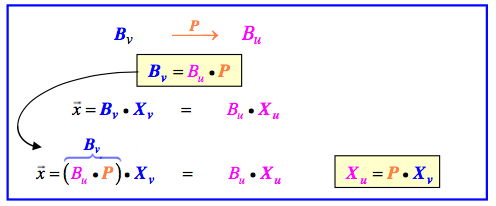
\includegraphics[width=\textwidth]{esquema}
\end{figure}
\end{frame}



 \begin{frame}
  \frametitle{Matriz de cambio de base}
\begin{block}{Matriz de cambio de base}
Dado un espacio vectorial de dimensi\'on $n$ y dos bases diferentes $B_u$ y $B_v$. Se denomina matriz de cambio de base de $B_v$ a $B_u$ a la matriz $P$ las columnas de la cual son las coordenadas de la base $B_v$ en la base $B_u$.
\end{block}
\end{frame}

 \begin{frame}
  \frametitle{Matriz de cambio de base}
\begin{block}{Ejercicios}
Dadas las bases $B_u = \{\vec u_1, \vec u_2, \vec u_3\}$ y $B_v = \{\vec v_1,\vec v_2,\vec v_3\}$, y el vector $\vec x$ de coordenadas $(2,1,0)$ en la base $B_v$, calc\'ulense sus coordenadas en la base $B_u$ sabiendo que:
\[\left\{\begin{array}{ccccccc}\vec v_1 & = & 2\vec u_1 & - & \vec u_2 & + & \vec u_3 \\\vec v_2 & = &  & - & \vec u_2 & + & 2\vec u_3 \\\vec v_3 & = & -\vec u_1 & + & \vec u_2 & - & 3\vec u_3\end{array}\right.\]
 \end{block}
\end{frame}

\begin{frame}
  \frametitle{Matriz de cambio de base}
Sol
\[P = \left(\begin{array}{ccc}
2&0&-1\\
-1&-1&1\\
1&2&-3
\end{array}\right)\]
Donde $B_v = B_u\cdot P$
\[\vec x = (4,-3,4)_{B_u}\]
\end{frame}

 \begin{frame}
  \frametitle{Matriz de cambio de base}
\begin{block}{Ejercicios}
Expr\'esese el vector $(-1,0,4)$ de la base can\'onica en la base $B=\{(1,3,-1),(-1,1,0),(0,2,0)\}$ de $\mathbb R^3$ calculando previamente la matriz de cambio de base necesaria.
 \end{block}
 Pista: $P$ es la matriz que porta la base can\'onica a $B$, la cual tiene como columnas los vectores de la base can\'onica expresados en la base $B$. este problema es m\'as sencillo si se busca la matriz $Q$ que porta $B$ a la base can\'onica (sus columnas ser\'an los vectores de $B$ en la base can\'onica que son ellos mismos) y que resulta ser la inversa de $P$.
\end{frame}

\begin{frame}
  \frametitle{Matriz de cambio de base}
Sol
\[P = Q^{-1} = \left(\begin{array}{ccc}
0&0&-1\\
-1&0&-1\\
1/2&1/2&2
\end{array}\right)\]
Donde $X_B = P\cdot X_{e}$
\[\vec x = \left(-4,-3,\frac{15}{2}\right)_{B}\]
\end{frame}


\section{Subespacios vectoriales}
\subsection{Concepto de subespacio vectorial}

 \begin{frame}
  \frametitle{Subespacio vectorial}
\begin{block}{Definici\'on}
Sea $F\subseteq E$ un subconjunto no vac\'io del espacio vectorial $E$ sobre un cuerpo $\mathbb K$. D\'icese que $F$ es un subespacio vectorial de $E$ si y solo si se verifica:
\begin{itemize}
\item La suma de dos elementos de $F$ es otro elemento $F$
\[\forall \vec x, \vec y\in F \Rightarrow \vec x +\vec y\in F\]
\item El producto de un escalar por un elemento $F$ es otro elemento de $F$
\[\forall \vec x \in F, \alpha\in \mathbb K \Rightarrow \alpha \vec x\in F\]
\end{itemize}
 \end{block}

\end{frame}


\begin{frame}
  \frametitle{Subespacio vectorial}
\begin{block}{Subespacios triviales}
Si $E$ es un $\mathbb K$-espacio vectorial, se verifica siempre que $E$ y $\{0\}$ son subespacios vectoriales de $E$. Se denominan subespacios vectoriales triviales o impropios. \end{block}
\begin{block}{Corolario}
Si $S$ es un subespacio vectorial de $E$, entonces $\vec 0\in S$. \end{block}

Este corolario solo se puede emplear rec\'iprocamente ya que si se comprueba que por alguna raz\'on $\vec 0\notin S$, entonces este conjunto no puede ser nunca un subespacio vectorial.
\end{frame}


\begin{frame}
  \frametitle{Subespacio vectorial}
\begin{block}{Ejercicios}
Compru\'ebese que el siguiente conjunto es un subespacio vectorial de $\mathbb R^3$:
\[F=\{(x,y,z)\in \mathbb R^3: x+y+z=0\}\]
Nota: compru\'ebese primero si $F$ contiene el vector cero y, si as\'i es, compru\'ebense las dos condiciones de la definici\'on de subespacio.
\end{block}

\end{frame}

\begin{frame}
  \frametitle{Subespacio vectorial}
\begin{block}{Ecuaciones de un subespacio vectorial}
Un subespacio vectorial $F$ de un espacio vectorial $E$ queda identificado si:
\begin{itemize}
\item Se conoce una base de $F$
\item Se conoce un sistema generador de $F$
\item A partir de sus ecuaciones par\'ametricas
\item A partir de las equacions cartesianas o impl\'icitas (un sistema homog\'eneo las inc\'ognitas del cual son las coordenadas del vector gen\'erico).
\end{itemize}
\end{block}
\end{frame}


\begin{frame}
  \frametitle{Subespacio vectorial}

\begin{block}{Ejercicios}
Identif\'iquese el subespacio $F$ del ejercicio anterior de todas las formas posibles:
\[F=\{(x,y,z)\in \mathbb R^3: x+y+z=0\}\]
\end{block}

\end{frame}

\begin{frame}
  \frametitle{Subespacio vectorial}
\begin{block}{Obtener una base de un subespacio vectorial}
\begin{itemize}
\item Se parte de las ecuaciones par\'ametricas del subespacio.
\item Se expresa el vector gen\'erico como combinaci\'on lineal de vectores.
	\begin{itemize}
	\item En primer lugar se consiguen tantos sumandos como par\'ametros tenga el subespacio y se separan en vectores diferentes
	\item Se extrae un escalar de cada uno de los vectores y se deja expresado como combinaci\'on lineal
	\end{itemize}
\item Los vectores que aparecen en la combinaci\'on lineal son un sistema generador del subespacio.
\item Se extrae del conjunto de vectores un subconjunto linealmente independiente con tantos vectores como indique el rango. Se tiene as\'i una base del subespacio.
\end{itemize}
\end{block}

\end{frame}


\begin{frame}
  \frametitle{Subespacio vectorial}
\begin{block}{Ejercicios}
Obt\'engase la dimensi\'on, las ecuaciones par\'ametricas y una base del subespacio $F_1$ dado por:
\[F_1=\{(x,y,z)\in\mathbb R^3: 2x-y+3z = 0, -x+y-z=0,x-2y=0\}\]
Pista: Comi\'encese por hacer Gauss al sistema de ecuaciones lineales.
\end{block}
\end{frame}


\begin{frame}
  \frametitle{Subespacio vectorial}
\begin{block}{Ejercicios}
Obt\'engase la dimensi\'on, las ecuaciones par\'ametricas y una base del subespacio $F_2$ dado por:
\[F_2=\{(\alpha+\beta,\alpha+\beta, \alpha+\beta+\gamma,0): \alpha, \beta, \gamma \in\mathbb R\}\]
Pista: Comi\'encese por hacer Gauss al sistema de ecuaciones lineales.
\end{block}
\end{frame}



\section{Bases ortogonales y ortonormales}
\begin{frame}
  \frametitle{Bases ortogonales y ortonormales}
\begin{block}{Base ortogonal}
Dada una base $B=\{\vec u_1,\vec u_2,\cdots,\vec u_n\}$ de un espacio vectorial $E$, d\'icese ortogonal si sus elementos son ortogonales dos a dos:
\[\vec u_i\cdot \vec u_j = 0 \forall i\neq j\]
\end{block}
\begin{block}{Base ortonormal}
Dada una base $B=\{\vec u_1,\vec u_2,\cdots,\vec u_n\}$ de un espacio vectorial $E$, d\'icese ortonormal si sus elementos son ortogonales dos a dos y adem\'as son unitarios:
\[\vec u_i\cdot \vec u_j = 0\ \forall i\neq j\]
\[\vec u_i\cdot \vec u_i = 1\ \forall i\]
\end{block}
\end{frame}

\subsection{M\'etodo de diagonalizaci\'on de Gram-Schmidt}
\begin{frame}
  \frametitle{M\'etodo de diagonalizaci\'on de Gram-Schmidt}
Este m\'etodo permite contruir una base ortogonal a partir de una base cualquiera del espacio vectorial. Primero se realizar\'a la contrucci\'on para un espacio vectorial de dos dimensiones:
\end{frame}

\begin{frame}
  \frametitle{M\'etodo de diagonalizaci\'on de Gram-Schmidt}
\begin{block}{Caso 2D}
Sea $B=\{\vec v_1,\vec v_2\}$ una base de un espacio vectorial de dos dimensiones. A partir de los vectores de esta base se construir\'a una nueva $B=\{\vec w_1,\vec w_2\}$ que ser\'a ortogonal y del mismo espacio.
\begin{enumerate}
\item Se toma $\vec w_1 = \vec v_1$ como primer vector de la nueva base.
\item El segundo vector ser\'a una combinaci\'on lineal $\vec v_1$ y $\vec v_2$ para asegurarse de que la nueva base genera el mismo subespacio vectorial. As\'i, se descompone:
\[\vec v_2 = \vec u_1+\vec u_2: \ \vec u_1||\vec v_1\ \ \vec u_2\perp\vec v_1\]
En particular $\vec u_2 = \vec v_2-t\vec v_1 = \vec v_2-t\vec w_1$ y ser\'a el siguiente vector de nuestra nueva base: $\vec w_2$. Solo resta encontrar $t$.
\end{enumerate}
\end{block}
\end{frame}


\begin{frame}
  \frametitle{M\'etodo de diagonalizaci\'on de Gram-Schmidt}
\begin{figure}[h]
  \label{fig:esquema}
\centering
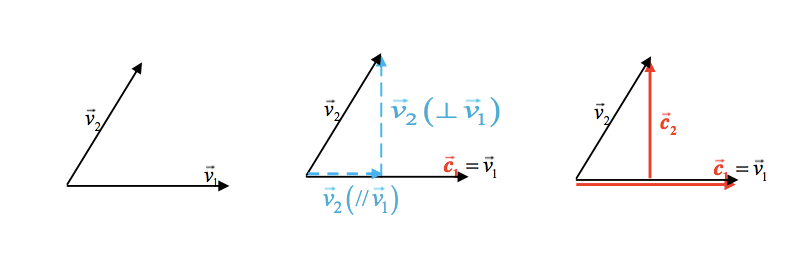
\includegraphics[width=\textwidth]{gram}
\end{figure}
\end{frame}

\begin{frame}
  \frametitle{M\'etodo de diagonalizaci\'on de Gram-Schmidt}
\begin{block}{Caso 2D}
Se tiene que $\vec w_1\perp\vec w_2$. Se impone la condici\'on de que $\vec w_2 = \vec v_2-t\vec w_1 $ y el producto escalar con $\vec w_1 = \vec v_1$ ha de ser cero:
\[\vec w_1\cdot \vec w_2 = \vec w_1\cdot (\vec v_2-t\vec w_1) = \vec w_1\cdot \vec v_2-\vec w_1\vec w_1 = 0 \]
Por lo tanto:
\[t = \frac{\vec w_1\cdot \vec v_2}{\vec w_1\cdot \vec w_1}\]
\[\vec w_2 = \vec v_2 - \frac{\vec w_1\cdot \vec v_2}{\vec w_1\cdot \vec w_1}\vec w_1\]
Entonces $B_r = \{\vec w_1,\vec w_2\}$ es una base ortogonal que genera el mismo subespacio que $B=\{\vec v_1, \vec v_2\}$.
\end{block}
\end{frame}


\begin{frame}
  \frametitle{M\'etodo de diagonalizaci\'on de Gram-Schmidt}
\begin{block}{Caso general}
Sea $B=\{\vec v_1,\vec v_2,\cdots, \vec v_n\}$ una base de un espacio vectorial de $n$ dimensiones $E$. A partir de los vectores de esta base se construir\'a una nueva $B_r=\{\vec w_1,\vec w_2,\cdots,\vec w_n\}$ que ser\'a ortogonal y del mismo espacio.
\begin{enumerate}
\item Se toma $\vec w_1 = \vec v_1$ como primer vector de la nueva base.
\item El segundo vector ser\'a una combinaci\'on lineal $\vec v_1$ y $\vec v_2$ de la forma $\vec w_2 = \vec v_2-t\vec w_1$, al cual se impondr\'a la condici\'on de que $\vec w_1\perp\vec w_2$. Operando se obtiene:
\end{enumerate}
\end{block}
\end{frame}



\begin{frame}
  \frametitle{M\'etodo de diagonalizaci\'on de Gram-Schmidt}
\begin{block}{Caso general}
\[t = \frac{\vec w_1\cdot \vec v_2}{\vec w_1\cdot \vec w_1}\]
\[\vec w_2 = \vec v_2 - \frac{\vec w_1\cdot \vec v_2}{\vec w_1\cdot \vec w_1}\vec w_1\]
\end{block}
\end{frame}

\begin{frame}
  \frametitle{M\'etodo de diagonalizaci\'on de Gram-Schmidt}
\begin{block}{Caso general}
Sea $B=\{\vec v_1,\vec v_2,\cdots, \vec v_n\}$ una base de un espacio vectorial de $n$ dimensiones $E$. A partir de los vectores de esta base se construir\'a una nueva $B_r=\{\vec w_1,\vec w_2,\cdots,\vec w_n\}$ que ser\'a ortogonal de $E$.
\begin{itemize}
\item[3] Para calcular el tercer vector, se procede de la misma forma: el tercer vector $\vec w_3$ ser\'a una combinaci\'on lineal de $\vec v_1, \vec v_2$ y $\vec v_3$ de la forma $\vec w_2 = \vec v_3-t_1\vec w_1-t_2\vec w_2$, a la cual se impondr\'an las condiciones $\vec w_1\perp\vec w_3$ i $\vec w_2\perp\vec w_3$  . Operando se obtiene:
\end{itemize}
\end{block}
\end{frame}


\begin{frame}
  \frametitle{M\'etodo de diagonalizaci\'on de Gram-Schmidt}
\begin{block}{Caso general}
\[t_1 = \frac{\vec w_1\cdot \vec v_3}{\vec w_1\cdot \vec w_1}\ \ t_2 = \frac{\vec w_2\cdot \vec v_2}{\vec w_2\cdot \vec w_2}\]
\[\vec w_3 = \vec v_3 - \frac{\vec w_1\cdot \vec v_3}{\vec w_1\cdot \vec w_1}\vec w_1 - \frac{\vec w_2\cdot \vec v_3}{\vec w_2\cdot \vec w_2}\vec w_2\]
\end{block}
\end{frame}


\begin{frame}
  \frametitle{M\'etodo de diagonalizaci\'on de Gram-Schmidt}
\begin{block}{Caso general}
\begin{itemize}
\item[4] An\'alogamente:
\[\vec w_4 = \vec v_4 - \frac{\vec w_1\cdot \vec v_4}{\vec w_1\cdot \vec w_1}\vec w_1 - \frac{\vec w_2\cdot \vec v_4}{\vec w_2\cdot \vec w_2}\vec w_2 - \frac{\vec w_3\cdot \vec v_4}{\vec w_3\cdot \vec w_3}\vec w_3\]
\item[n] Y con el fin de hallar el \'ultimo:
\[\vec w_n = \vec v_n - \sum_{i=1}^{n-1} \frac{\vec w_i\cdot \vec v_n}{\vec w_i\cdot \vec w_i}\vec w_i\]
\item[n+1] Finalmente, si se designa una base ortonormal, basta dividir cada vector por su norma. 
\end{itemize}
\end{block}
\end{frame}


\begin{frame}
  \frametitle{M\'etodo de diagonalizaci\'on de Gram-Schmidt}
\begin{block}{Ejercicios}
Calc\'ulese una base ortogonal del subespacio vectorial generado por los vectores
\[\vec u_1 = (1,1,0,1), \vec u_2 = (0,0,1,1), \vec u_3 = (2,0,-1,0)\]
\end{block}
Sol: 
\[(1,1,0,1),(1,1,-3,-2),(1,-1,0,0)\]
\end{frame}

\subsection{Proyecci\'on ortogonal de un vector sobre un subespacio}
\begin{frame}
  \frametitle{Vector ortogonal a un subespacio}
\begin{block}{Vector ortogonal a un subespacio}
Un vector $\vec u\in E$ es ortogonal a un subespacio vectorial $S\subseteq E$ si y solo si: 
\[\vec u \cdot \vec x = 0\ \forall\ \vec x \in S\]
\end{block}

\begin{block}{Teorema}
Un vector $\vec u\in E$ es ortogonal a un subespacio vectorial $S\subseteq E$ si y solo si es ortogonal a todos los vectores de una base de $S$.
\end{block}
\end{frame}

\begin{frame}
  \frametitle{Proyecci\'on ortogonal de un vector sobre un subespacio}
\begin{figure}[h]
  \label{fig:esquema}
\centering
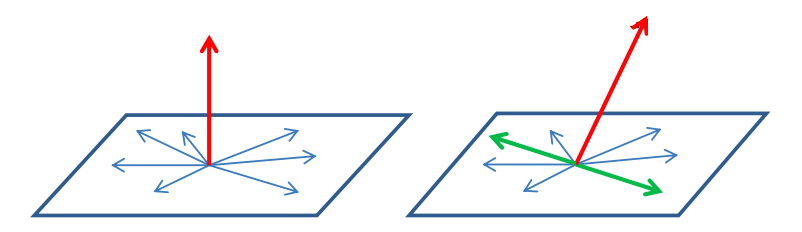
\includegraphics[width=\textwidth]{ortogonal}
\end{figure}
\end{frame}




\begin{frame}
  \frametitle{Proyecci\'on ortogonal de un vector sobre un subespacio}
\begin{block}{Teorema}
Dos subespacios $V$ y $W$ de $E$ son ortogonales si: 
\[\forall \vec x\in V\ \ \forall \vec y \in W \Rightarrow \vec x \cdot \vec y = 0\]
\end{block}

\begin{block}{Teorema}
Para que dos subespacios $V$ y $W$ sean ortogonales, es suficiente con que los vectores de una base de $V$ sean ortogonales a los vectores de una base de $W$.
\end{block}
\end{frame}

\begin{frame}
  \frametitle{Proyecci\'on ortogonal de un vector sobre un subespacio}
\begin{figure}[h]
  \label{fig:esquema}
\centering
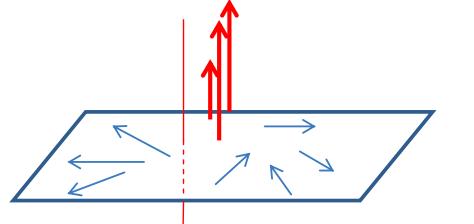
\includegraphics[width=\textwidth]{ortogonal2}
\end{figure}
\end{frame}





\begin{frame}
  \frametitle{Proyecci\'on ortogonal de un vector sobre un subespacio}
\begin{block}{Projecci\'on ortogonal }
Como se recordar\'a, el vector proyecci\'on ortogonal de un vector $\vec u$ sobre otro $\vec v$, se expresa como:
\[P_{\vec u}(\vec v) = \frac{\vec u\cdot \vec v}{\vec v\cdot \vec v}\vec v = \frac{\vec u \cdot \vec v}{||\vec v||^2}\vec v\]
\end{block}
\end{frame}


\begin{frame}
  \frametitle{Proyecci\'on ortogonal de un vector sobre un subespacio}
\begin{block}{Proyecci\'on ortogonal de un vector sobre un subespacio}
Dado $S$ un subespacio vectorial de un espacio vectorial $E$, todo vector $\vec u\in E$  se descompone de manera \'unica en: 
\[\vec u = \vec u_S+\vec u_0\]
Con $\vec u_S \in S$ y $\vec u_0\in S^\perp$. En particular, el vector $\vec u_S\in S$ se denomina vector proyecci\'on ortogonal de $\vec u$ sobre $S$.
\end{block}
\end{frame}




\begin{frame}
  \frametitle{Proyecci\'on ortogonal de un vector sobre un subespacio}
\begin{block}{Proyecci\'on ortogonal de un vector sobre un subespacio}
Si se toma en $S$ una base ortogonal $\{\vec s_1,\vec s_2,\cdots,\vec s_r\}$, la proyecci\'on de $\vec u$ sobre $S$ viene dada por:
\[P_{\vec u}(\vec v) = \vec u_S = \sum_{i=1}^r \frac{\vec u \cdot \vec s_i}{||\vec s_i||^2}\vec s_i\]
\end{block}
\end{frame}

%  \begin{figure}[h]
  %  \label{fig:volumen}
%\centering
%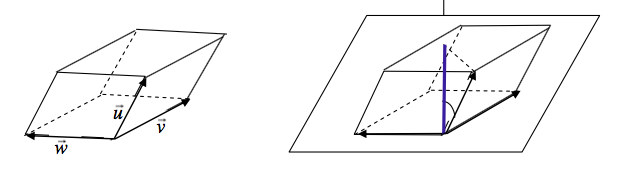
\includegraphics[height=3cm]{volum}
%\end{figure}


\end{document}